% Created by tikzDevice version 0.12.6 on 2024-03-22 09:45:18
% !TEX encoding = UTF-8 Unicode
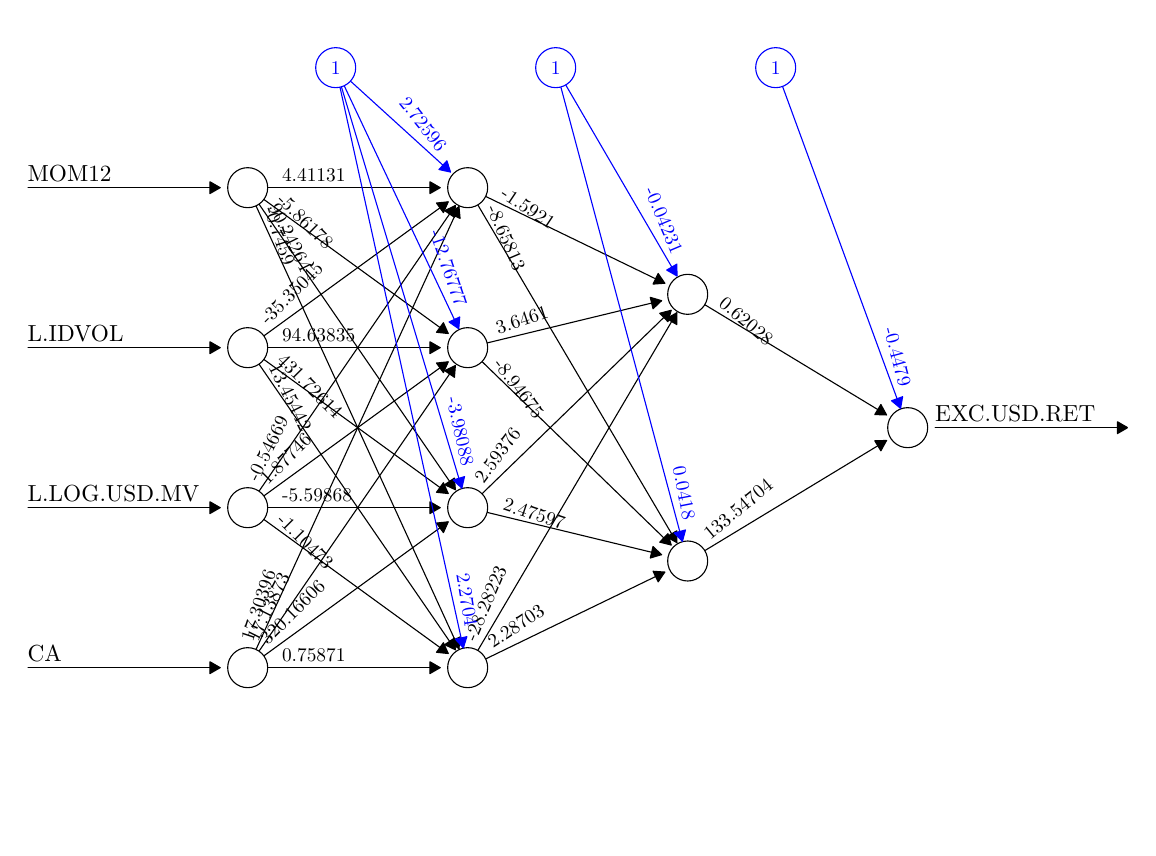
\begin{tikzpicture}[x=1pt,y=1pt]
\definecolor{fillColor}{RGB}{255,255,255}
\path[use as bounding box,fill=fillColor,fill opacity=0.00] (0,0) rectangle (397.48,289.08);
\begin{scope}
\path[clip] (  0.00,  0.00) rectangle (397.48,289.08);
\definecolor{drawColor}{RGB}{0,0,0}

\path[draw=drawColor,line width= 0.4pt,line join=round,line cap=round] ( 79.50, 57.82) --
	(149.06, 57.82);
\definecolor{fillColor}{RGB}{0,0,0}

\path[draw=drawColor,line width= 0.4pt,line join=round,line cap=round,fill=fillColor] (145.36, 55.68) --
	(149.06, 57.82) --
	(145.36, 59.95) --
	cycle;

\node[text=drawColor,anchor=base west,inner sep=0pt, outer sep=0pt, scale=  0.70] at ( 91.92, 59.95) {0.75871};
\end{scope}
\begin{scope}
\path[clip] (  0.00,  0.00) rectangle (397.48,289.08);
\definecolor{drawColor}{RGB}{0,0,0}

\path[draw=drawColor,line width= 0.4pt,line join=round,line cap=round] ( 79.50, 57.82) --
	(151.97,110.52);
\definecolor{fillColor}{RGB}{0,0,0}

\path[draw=drawColor,line width= 0.4pt,line join=round,line cap=round,fill=fillColor] (150.23,106.62) --
	(151.97,110.52) --
	(147.72,110.07) --
	cycle;

\node[text=drawColor,rotate= 45.00,anchor=base west,inner sep=0pt, outer sep=0pt, scale=  0.70] at ( 86.77, 65.71) {320.16606};
\end{scope}
\begin{scope}
\path[clip] (  0.00,  0.00) rectangle (397.48,289.08);
\definecolor{drawColor}{RGB}{0,0,0}

\path[draw=drawColor,line width= 0.4pt,line join=round,line cap=round] ( 79.50, 57.82) --
	(154.55,166.98);
\definecolor{fillColor}{RGB}{0,0,0}

\path[draw=drawColor,line width= 0.4pt,line join=round,line cap=round,fill=fillColor] (154.21,162.73) --
	(154.55,166.98) --
	(150.70,165.15) --
	cycle;

\node[text=drawColor,rotate= 63.43,anchor=base west,inner sep=0pt, outer sep=0pt, scale=  0.70] at ( 83.14, 66.85) {17.13873};
\end{scope}
\begin{scope}
\path[clip] (  0.00,  0.00) rectangle (397.48,289.08);
\definecolor{drawColor}{RGB}{0,0,0}

\path[draw=drawColor,line width= 0.4pt,line join=round,line cap=round] ( 79.50, 57.82) --
	(155.85,224.41);
\definecolor{fillColor}{RGB}{0,0,0}

\path[draw=drawColor,line width= 0.4pt,line join=round,line cap=round,fill=fillColor] (156.25,220.16) --
	(155.85,224.41) --
	(152.37,221.94) --
	cycle;

\node[text=drawColor,rotate= 71.57,anchor=base west,inner sep=0pt, outer sep=0pt, scale=  0.70] at ( 81.40, 67.06) {17.30396};
\end{scope}
\begin{scope}
\path[clip] (  0.00,  0.00) rectangle (397.48,289.08);
\definecolor{drawColor}{RGB}{0,0,0}

\path[draw=drawColor,line width= 0.4pt,line join=round,line cap=round] ( -0.00, 57.82) --
	( 69.56, 57.82);
\definecolor{fillColor}{RGB}{0,0,0}

\path[draw=drawColor,line width= 0.4pt,line join=round,line cap=round,fill=fillColor] ( 65.86, 55.68) --
	( 69.56, 57.82) --
	( 65.86, 59.95) --
	cycle;

\node[text=drawColor,anchor=base west,inner sep=0pt, outer sep=0pt, scale=  0.84] at ( -0.00, 59.95) {CA};
\end{scope}
\begin{scope}
\path[clip] (  0.00,  0.00) rectangle (397.48,289.08);
\definecolor{drawColor}{RGB}{0,0,0}
\definecolor{fillColor}{RGB}{255,255,255}

\path[draw=drawColor,line width= 0.4pt,line join=round,line cap=round,fill=fillColor] ( 79.50, 57.82) circle (  7.23);

\path[draw=drawColor,line width= 0.4pt,line join=round,line cap=round] ( 79.50,115.63) --
	(151.97, 62.93);
\definecolor{fillColor}{RGB}{0,0,0}

\path[draw=drawColor,line width= 0.4pt,line join=round,line cap=round,fill=fillColor] (147.72, 63.37) --
	(151.97, 62.93) --
	(150.23, 66.83) --
	cycle;

\node[text=drawColor,rotate=-45.00,anchor=base west,inner sep=0pt, outer sep=0pt, scale=  0.70] at ( 89.79,110.75) {-1.10473};
\end{scope}
\begin{scope}
\path[clip] (  0.00,  0.00) rectangle (397.48,289.08);
\definecolor{drawColor}{RGB}{0,0,0}

\path[draw=drawColor,line width= 0.4pt,line join=round,line cap=round] ( 79.50,115.63) --
	(149.06,115.63);
\definecolor{fillColor}{RGB}{0,0,0}

\path[draw=drawColor,line width= 0.4pt,line join=round,line cap=round,fill=fillColor] (145.36,113.50) --
	(149.06,115.63) --
	(145.36,117.77) --
	cycle;

\node[text=drawColor,anchor=base west,inner sep=0pt, outer sep=0pt, scale=  0.70] at ( 91.92,117.77) {-5.59868};
\end{scope}
\begin{scope}
\path[clip] (  0.00,  0.00) rectangle (397.48,289.08);
\definecolor{drawColor}{RGB}{0,0,0}

\path[draw=drawColor,line width= 0.4pt,line join=round,line cap=round] ( 79.50,115.63) --
	(151.97,168.34);
\definecolor{fillColor}{RGB}{0,0,0}

\path[draw=drawColor,line width= 0.4pt,line join=round,line cap=round,fill=fillColor] (150.23,164.44) --
	(151.97,168.34) --
	(147.72,167.89) --
	cycle;

\node[text=drawColor,rotate= 45.00,anchor=base west,inner sep=0pt, outer sep=0pt, scale=  0.70] at ( 86.77,123.53) {1.87746};
\end{scope}
\begin{scope}
\path[clip] (  0.00,  0.00) rectangle (397.48,289.08);
\definecolor{drawColor}{RGB}{0,0,0}

\path[draw=drawColor,line width= 0.4pt,line join=round,line cap=round] ( 79.50,115.63) --
	(154.55,224.80);
\definecolor{fillColor}{RGB}{0,0,0}

\path[draw=drawColor,line width= 0.4pt,line join=round,line cap=round,fill=fillColor] (154.21,220.55) --
	(154.55,224.80) --
	(150.70,222.96) --
	cycle;

\node[text=drawColor,rotate= 63.43,anchor=base west,inner sep=0pt, outer sep=0pt, scale=  0.70] at ( 83.14,124.67) {-0.54669};
\end{scope}
\begin{scope}
\path[clip] (  0.00,  0.00) rectangle (397.48,289.08);
\definecolor{drawColor}{RGB}{0,0,0}

\path[draw=drawColor,line width= 0.4pt,line join=round,line cap=round] ( -0.00,115.63) --
	( 69.56,115.63);
\definecolor{fillColor}{RGB}{0,0,0}

\path[draw=drawColor,line width= 0.4pt,line join=round,line cap=round,fill=fillColor] ( 65.86,113.50) --
	( 69.56,115.63) --
	( 65.86,117.77) --
	cycle;

\node[text=drawColor,anchor=base west,inner sep=0pt, outer sep=0pt, scale=  0.84] at ( -0.00,117.77) {L.LOG.USD.MV};
\end{scope}
\begin{scope}
\path[clip] (  0.00,  0.00) rectangle (397.48,289.08);
\definecolor{drawColor}{RGB}{0,0,0}
\definecolor{fillColor}{RGB}{255,255,255}

\path[draw=drawColor,line width= 0.4pt,line join=round,line cap=round,fill=fillColor] ( 79.50,115.63) circle (  7.23);

\path[draw=drawColor,line width= 0.4pt,line join=round,line cap=round] ( 79.50,173.45) --
	(154.55, 64.28);
\definecolor{fillColor}{RGB}{0,0,0}

\path[draw=drawColor,line width= 0.4pt,line join=round,line cap=round,fill=fillColor] (150.70, 66.12) --
	(154.55, 64.28) --
	(154.21, 68.53) --
	cycle;

\node[text=drawColor,rotate=-63.43,anchor=base west,inner sep=0pt, outer sep=0pt, scale=  0.70] at ( 86.96,166.32) {13.45442};
\end{scope}
\begin{scope}
\path[clip] (  0.00,  0.00) rectangle (397.48,289.08);
\definecolor{drawColor}{RGB}{0,0,0}

\path[draw=drawColor,line width= 0.4pt,line join=round,line cap=round] ( 79.50,173.45) --
	(151.97,120.74);
\definecolor{fillColor}{RGB}{0,0,0}

\path[draw=drawColor,line width= 0.4pt,line join=round,line cap=round,fill=fillColor] (147.72,121.19) --
	(151.97,120.74) --
	(150.23,124.64) --
	cycle;

\node[text=drawColor,rotate=-45.00,anchor=base west,inner sep=0pt, outer sep=0pt, scale=  0.70] at ( 89.79,168.57) {431.72614};
\end{scope}
\begin{scope}
\path[clip] (  0.00,  0.00) rectangle (397.48,289.08);
\definecolor{drawColor}{RGB}{0,0,0}

\path[draw=drawColor,line width= 0.4pt,line join=round,line cap=round] ( 79.50,173.45) --
	(149.06,173.45);
\definecolor{fillColor}{RGB}{0,0,0}

\path[draw=drawColor,line width= 0.4pt,line join=round,line cap=round,fill=fillColor] (145.36,171.31) --
	(149.06,173.45) --
	(145.36,175.58) --
	cycle;

\node[text=drawColor,anchor=base west,inner sep=0pt, outer sep=0pt, scale=  0.70] at ( 91.92,175.58) {94.63835};
\end{scope}
\begin{scope}
\path[clip] (  0.00,  0.00) rectangle (397.48,289.08);
\definecolor{drawColor}{RGB}{0,0,0}

\path[draw=drawColor,line width= 0.4pt,line join=round,line cap=round] ( 79.50,173.45) --
	(151.97,226.15);
\definecolor{fillColor}{RGB}{0,0,0}

\path[draw=drawColor,line width= 0.4pt,line join=round,line cap=round,fill=fillColor] (150.23,222.25) --
	(151.97,226.15) --
	(147.72,225.71) --
	cycle;

\node[text=drawColor,rotate= 45.00,anchor=base west,inner sep=0pt, outer sep=0pt, scale=  0.70] at ( 86.77,181.34) {-35.35045};
\end{scope}
\begin{scope}
\path[clip] (  0.00,  0.00) rectangle (397.48,289.08);
\definecolor{drawColor}{RGB}{0,0,0}

\path[draw=drawColor,line width= 0.4pt,line join=round,line cap=round] ( -0.00,173.45) --
	( 69.56,173.45);
\definecolor{fillColor}{RGB}{0,0,0}

\path[draw=drawColor,line width= 0.4pt,line join=round,line cap=round,fill=fillColor] ( 65.86,171.31) --
	( 69.56,173.45) --
	( 65.86,175.58) --
	cycle;

\node[text=drawColor,anchor=base west,inner sep=0pt, outer sep=0pt, scale=  0.84] at ( -0.00,175.58) {L.IDVOL};
\end{scope}
\begin{scope}
\path[clip] (  0.00,  0.00) rectangle (397.48,289.08);
\definecolor{drawColor}{RGB}{0,0,0}
\definecolor{fillColor}{RGB}{255,255,255}

\path[draw=drawColor,line width= 0.4pt,line join=round,line cap=round,fill=fillColor] ( 79.50,173.45) circle (  7.23);

\path[draw=drawColor,line width= 0.4pt,line join=round,line cap=round] ( 79.50,231.26) --
	(155.85, 64.67);
\definecolor{fillColor}{RGB}{0,0,0}

\path[draw=drawColor,line width= 0.4pt,line join=round,line cap=round,fill=fillColor] (152.37, 67.14) --
	(155.85, 64.67) --
	(156.25, 68.92) --
	cycle;

\node[text=drawColor,rotate=-71.57,anchor=base west,inner sep=0pt, outer sep=0pt, scale=  0.70] at ( 85.45,223.37) {-0.7459};
\end{scope}
\begin{scope}
\path[clip] (  0.00,  0.00) rectangle (397.48,289.08);
\definecolor{drawColor}{RGB}{0,0,0}

\path[draw=drawColor,line width= 0.4pt,line join=round,line cap=round] ( 79.50,231.26) --
	(154.55,122.10);
\definecolor{fillColor}{RGB}{0,0,0}

\path[draw=drawColor,line width= 0.4pt,line join=round,line cap=round,fill=fillColor] (150.70,123.93) --
	(154.55,122.10) --
	(154.21,126.35) --
	cycle;

\node[text=drawColor,rotate=-63.43,anchor=base west,inner sep=0pt, outer sep=0pt, scale=  0.70] at ( 86.96,224.14) {90.24264};
\end{scope}
\begin{scope}
\path[clip] (  0.00,  0.00) rectangle (397.48,289.08);
\definecolor{drawColor}{RGB}{0,0,0}

\path[draw=drawColor,line width= 0.4pt,line join=round,line cap=round] ( 79.50,231.26) --
	(151.97,178.56);
\definecolor{fillColor}{RGB}{0,0,0}

\path[draw=drawColor,line width= 0.4pt,line join=round,line cap=round,fill=fillColor] (147.72,179.01) --
	(151.97,178.56) --
	(150.23,182.46) --
	cycle;

\node[text=drawColor,rotate=-45.00,anchor=base west,inner sep=0pt, outer sep=0pt, scale=  0.70] at ( 89.79,226.39) {-5.86178};
\end{scope}
\begin{scope}
\path[clip] (  0.00,  0.00) rectangle (397.48,289.08);
\definecolor{drawColor}{RGB}{0,0,0}

\path[draw=drawColor,line width= 0.4pt,line join=round,line cap=round] ( 79.50,231.26) --
	(149.06,231.26);
\definecolor{fillColor}{RGB}{0,0,0}

\path[draw=drawColor,line width= 0.4pt,line join=round,line cap=round,fill=fillColor] (145.36,229.13) --
	(149.06,231.26) --
	(145.36,233.40) --
	cycle;

\node[text=drawColor,anchor=base west,inner sep=0pt, outer sep=0pt, scale=  0.70] at ( 91.92,233.40) {4.41131};
\end{scope}
\begin{scope}
\path[clip] (  0.00,  0.00) rectangle (397.48,289.08);
\definecolor{drawColor}{RGB}{0,0,0}

\path[draw=drawColor,line width= 0.4pt,line join=round,line cap=round] ( -0.00,231.26) --
	( 69.56,231.26);
\definecolor{fillColor}{RGB}{0,0,0}

\path[draw=drawColor,line width= 0.4pt,line join=round,line cap=round,fill=fillColor] ( 65.86,229.13) --
	( 69.56,231.26) --
	( 65.86,233.40) --
	cycle;

\node[text=drawColor,anchor=base west,inner sep=0pt, outer sep=0pt, scale=  0.84] at ( -0.00,233.40) {MOM12};
\end{scope}
\begin{scope}
\path[clip] (  0.00,  0.00) rectangle (397.48,289.08);
\definecolor{drawColor}{RGB}{0,0,0}
\definecolor{fillColor}{RGB}{255,255,255}

\path[draw=drawColor,line width= 0.4pt,line join=round,line cap=round,fill=fillColor] ( 79.50,231.26) circle (  7.23);

\path[draw=drawColor,line width= 0.4pt,line join=round,line cap=round] (158.99, 57.82) --
	(230.22, 92.35);
\definecolor{fillColor}{RGB}{0,0,0}

\path[draw=drawColor,line width= 0.4pt,line join=round,line cap=round,fill=fillColor] (227.83, 88.82) --
	(230.22, 92.35) --
	(225.97, 92.66) --
	cycle;

\node[text=drawColor,rotate= 33.69,anchor=base west,inner sep=0pt, outer sep=0pt, scale=  0.70] at (168.15, 64.60) {2.28703};
\end{scope}
\begin{scope}
\path[clip] (  0.00,  0.00) rectangle (397.48,289.08);
\definecolor{drawColor}{RGB}{0,0,0}

\path[draw=drawColor,line width= 0.4pt,line join=round,line cap=round] (158.99, 57.82) --
	(234.58,186.08);
\definecolor{fillColor}{RGB}{0,0,0}

\path[draw=drawColor,line width= 0.4pt,line join=round,line cap=round,fill=fillColor] (234.54,181.81) --
	(234.58,186.08) --
	(230.86,183.98) --
	cycle;

\node[text=drawColor,rotate= 66.80,anchor=base west,inner sep=0pt, outer sep=0pt, scale=  0.70] at (161.93, 66.96) {-28.28223};
\end{scope}
\begin{scope}
\path[clip] (  0.00,  0.00) rectangle (397.48,289.08);
\definecolor{drawColor}{RGB}{0,0,0}
\definecolor{fillColor}{RGB}{255,255,255}

\path[draw=drawColor,line width= 0.4pt,line join=round,line cap=round,fill=fillColor] (158.99, 57.82) circle (  7.23);

\path[draw=drawColor,line width= 0.4pt,line join=round,line cap=round] (158.99,115.63) --
	(229.06, 98.65);
\definecolor{fillColor}{RGB}{0,0,0}

\path[draw=drawColor,line width= 0.4pt,line join=round,line cap=round,fill=fillColor] (224.97, 97.44) --
	(229.06, 98.65) --
	(225.97,101.59) --
	cycle;

\node[text=drawColor,rotate=-18.43,anchor=base west,inner sep=0pt, outer sep=0pt, scale=  0.70] at (171.45,114.80) {2.47597};
\end{scope}
\begin{scope}
\path[clip] (  0.00,  0.00) rectangle (397.48,289.08);
\definecolor{drawColor}{RGB}{0,0,0}

\path[draw=drawColor,line width= 0.4pt,line join=round,line cap=round] (158.99,115.63) --
	(232.53,186.94);
\definecolor{fillColor}{RGB}{0,0,0}

\path[draw=drawColor,line width= 0.4pt,line join=round,line cap=round,fill=fillColor] (231.36,182.83) --
	(232.53,186.94) --
	(228.39,185.90) --
	cycle;

\node[text=drawColor,rotate= 53.13,anchor=base west,inner sep=0pt, outer sep=0pt, scale=  0.70] at (164.74,124.14) {2.59376};
\end{scope}
\begin{scope}
\path[clip] (  0.00,  0.00) rectangle (397.48,289.08);
\definecolor{drawColor}{RGB}{0,0,0}
\definecolor{fillColor}{RGB}{255,255,255}

\path[draw=drawColor,line width= 0.4pt,line join=round,line cap=round,fill=fillColor] (158.99,115.63) circle (  7.23);

\path[draw=drawColor,line width= 0.4pt,line join=round,line cap=round] (158.99,173.45) --
	(232.53,102.14);
\definecolor{fillColor}{RGB}{0,0,0}

\path[draw=drawColor,line width= 0.4pt,line join=round,line cap=round,fill=fillColor] (228.39,103.18) --
	(232.53,102.14) --
	(231.36,106.25) --
	cycle;

\node[text=drawColor,rotate=-53.13,anchor=base west,inner sep=0pt, outer sep=0pt, scale=  0.70] at (168.15,167.50) {-8.94675};
\end{scope}
\begin{scope}
\path[clip] (  0.00,  0.00) rectangle (397.48,289.08);
\definecolor{drawColor}{RGB}{0,0,0}

\path[draw=drawColor,line width= 0.4pt,line join=round,line cap=round] (158.99,173.45) --
	(229.06,190.43);
\definecolor{fillColor}{RGB}{0,0,0}

\path[draw=drawColor,line width= 0.4pt,line join=round,line cap=round,fill=fillColor] (225.97,187.49) --
	(229.06,190.43) --
	(224.97,191.64) --
	cycle;

\node[text=drawColor,rotate= 18.43,anchor=base west,inner sep=0pt, outer sep=0pt, scale=  0.70] at (170.10,178.33) {3.6461};
\end{scope}
\begin{scope}
\path[clip] (  0.00,  0.00) rectangle (397.48,289.08);
\definecolor{drawColor}{RGB}{0,0,0}
\definecolor{fillColor}{RGB}{255,255,255}

\path[draw=drawColor,line width= 0.4pt,line join=round,line cap=round,fill=fillColor] (158.99,173.45) circle (  7.23);

\path[draw=drawColor,line width= 0.4pt,line join=round,line cap=round] (158.99,231.26) --
	(234.58,103.00);
\definecolor{fillColor}{RGB}{0,0,0}

\path[draw=drawColor,line width= 0.4pt,line join=round,line cap=round,fill=fillColor] (230.86,105.10) --
	(234.58,103.00) --
	(234.54,107.27) --
	cycle;

\node[text=drawColor,rotate=-66.80,anchor=base west,inner sep=0pt, outer sep=0pt, scale=  0.70] at (165.85,223.80) {-8.65813};
\end{scope}
\begin{scope}
\path[clip] (  0.00,  0.00) rectangle (397.48,289.08);
\definecolor{drawColor}{RGB}{0,0,0}

\path[draw=drawColor,line width= 0.4pt,line join=round,line cap=round] (158.99,231.26) --
	(230.22,196.73);
\definecolor{fillColor}{RGB}{0,0,0}

\path[draw=drawColor,line width= 0.4pt,line join=round,line cap=round,fill=fillColor] (225.97,196.42) --
	(230.22,196.73) --
	(227.83,200.26) --
	cycle;

\node[text=drawColor,rotate=-33.69,anchor=base west,inner sep=0pt, outer sep=0pt, scale=  0.70] at (170.51,228.03) {-1.5921};
\end{scope}
\begin{scope}
\path[clip] (  0.00,  0.00) rectangle (397.48,289.08);
\definecolor{drawColor}{RGB}{0,0,0}
\definecolor{fillColor}{RGB}{255,255,255}

\path[draw=drawColor,line width= 0.4pt,line join=round,line cap=round,fill=fillColor] (158.99,231.26) circle (  7.23);

\path[draw=drawColor,line width= 0.4pt,line join=round,line cap=round] (238.49, 96.36) --
	(310.35,139.91);
\definecolor{fillColor}{RGB}{0,0,0}

\path[draw=drawColor,line width= 0.4pt,line join=round,line cap=round,fill=fillColor] (308.30,136.17) --
	(310.35,139.91) --
	(306.09,139.82) --
	cycle;

\node[text=drawColor,rotate= 39.81,anchor=base west,inner sep=0pt, outer sep=0pt, scale=  0.70] at (246.67,103.78) {133.54704};
\end{scope}
\begin{scope}
\path[clip] (  0.00,  0.00) rectangle (397.48,289.08);
\definecolor{drawColor}{RGB}{0,0,0}
\definecolor{fillColor}{RGB}{255,255,255}

\path[draw=drawColor,line width= 0.4pt,line join=round,line cap=round,fill=fillColor] (238.49, 96.36) circle (  7.23);

\path[draw=drawColor,line width= 0.4pt,line join=round,line cap=round] (238.49,192.72) --
	(310.35,149.17);
\definecolor{fillColor}{RGB}{0,0,0}

\path[draw=drawColor,line width= 0.4pt,line join=round,line cap=round,fill=fillColor] (306.09,149.26) --
	(310.35,149.17) --
	(308.30,152.91) --
	cycle;

\node[text=drawColor,rotate=-39.81,anchor=base west,inner sep=0pt, outer sep=0pt, scale=  0.70] at (249.40,188.58) {0.62028};
\end{scope}
\begin{scope}
\path[clip] (  0.00,  0.00) rectangle (397.48,289.08);
\definecolor{drawColor}{RGB}{0,0,0}
\definecolor{fillColor}{RGB}{255,255,255}

\path[draw=drawColor,line width= 0.4pt,line join=round,line cap=round,fill=fillColor] (238.49,192.72) circle (  7.23);

\path[draw=drawColor,line width= 0.4pt,line join=round,line cap=round] (327.93,144.54) --
	(397.48,144.54);
\definecolor{fillColor}{RGB}{0,0,0}

\path[draw=drawColor,line width= 0.4pt,line join=round,line cap=round,fill=fillColor] (393.79,142.41) --
	(397.48,144.54) --
	(393.79,146.67) --
	cycle;

\node[text=drawColor,anchor=base west,inner sep=0pt, outer sep=0pt, scale=  0.84] at (327.93,146.67) {EXC.USD.RET};
\end{scope}
\begin{scope}
\path[clip] (  0.00,  0.00) rectangle (397.48,289.08);
\definecolor{drawColor}{RGB}{0,0,0}
\definecolor{fillColor}{RGB}{255,255,255}

\path[draw=drawColor,line width= 0.4pt,line join=round,line cap=round,fill=fillColor] (317.99,144.54) circle (  7.23);
\definecolor{drawColor}{RGB}{0,0,255}

\path[draw=drawColor,line width= 0.4pt,line join=round,line cap=round] (111.30,274.63) --
	(157.42, 64.95);
\definecolor{fillColor}{RGB}{0,0,255}

\path[draw=drawColor,line width= 0.4pt,line join=round,line cap=round,fill=fillColor] (154.55, 68.10) --
	(157.42, 64.95) --
	(158.71, 69.02) --
	cycle;

\node[text=drawColor,rotate=-80.91,anchor=base east,inner sep=0pt, outer sep=0pt, scale=  0.70] at (157.96, 72.43) {2.2704};
\end{scope}
\begin{scope}
\path[clip] (  0.00,  0.00) rectangle (397.48,289.08);
\definecolor{drawColor}{RGB}{0,0,255}

\path[draw=drawColor,line width= 0.4pt,line join=round,line cap=round] (111.30,274.63) --
	(156.88,122.69);
\definecolor{fillColor}{RGB}{0,0,255}

\path[draw=drawColor,line width= 0.4pt,line join=round,line cap=round,fill=fillColor] (153.77,125.62) --
	(156.88,122.69) --
	(157.86,126.85) --
	cycle;

\node[text=drawColor,rotate=-77.69,anchor=base east,inner sep=0pt, outer sep=0pt, scale=  0.70] at (156.84,130.21) {-3.98088};
\end{scope}
\begin{scope}
\path[clip] (  0.00,  0.00) rectangle (397.48,289.08);
\definecolor{drawColor}{RGB}{0,0,255}

\path[draw=drawColor,line width= 0.4pt,line join=round,line cap=round] (111.30,274.63) --
	(155.77,180.28);
\definecolor{fillColor}{RGB}{0,0,255}

\path[draw=drawColor,line width= 0.4pt,line join=round,line cap=round,fill=fillColor] (152.26,182.72) --
	(155.77,180.28) --
	(156.13,184.54) --
	cycle;

\node[text=drawColor,rotate=-71.08,anchor=base east,inner sep=0pt, outer sep=0pt, scale=  0.70] at (154.57,187.81) {-12.76777};
\end{scope}
\begin{scope}
\path[clip] (  0.00,  0.00) rectangle (397.48,289.08);
\definecolor{drawColor}{RGB}{0,0,255}

\path[draw=drawColor,line width= 0.4pt,line join=round,line cap=round] (111.30,274.63) --
	(152.79,236.91);
\definecolor{fillColor}{RGB}{0,0,255}

\path[draw=drawColor,line width= 0.4pt,line join=round,line cap=round,fill=fillColor] (148.62,237.81) --
	(152.79,236.91) --
	(151.49,240.97) --
	cycle;

\node[text=drawColor,rotate=-51.34,anchor=base east,inner sep=0pt, outer sep=0pt, scale=  0.70] at (148.24,243.88) {2.72596};
\end{scope}
\begin{scope}
\path[clip] (  0.00,  0.00) rectangle (397.48,289.08);
\definecolor{drawColor}{RGB}{0,0,255}
\definecolor{fillColor}{RGB}{255,255,255}

\path[draw=drawColor,line width= 0.4pt,line join=round,line cap=round,fill=fillColor] (111.30,274.63) circle (  7.23);

\node[text=drawColor,anchor=base,inner sep=0pt, outer sep=0pt, scale=  0.70] at (111.30,272.22) {1};

\path[draw=drawColor,line width= 0.4pt,line join=round,line cap=round] (190.79,274.63) --
	(236.59,103.45);
\definecolor{fillColor}{RGB}{0,0,255}

\path[draw=drawColor,line width= 0.4pt,line join=round,line cap=round,fill=fillColor] (233.58,106.47) --
	(236.59,103.45) --
	(237.70,107.58) --
	cycle;

\node[text=drawColor,rotate=-78.99,anchor=base east,inner sep=0pt, outer sep=0pt, scale=  0.70] at (236.79,110.96) {0.0418};
\end{scope}
\begin{scope}
\path[clip] (  0.00,  0.00) rectangle (397.48,289.08);
\definecolor{drawColor}{RGB}{0,0,255}

\path[draw=drawColor,line width= 0.4pt,line join=round,line cap=round] (190.79,274.63) --
	(234.62,199.37);
\definecolor{fillColor}{RGB}{0,0,255}

\path[draw=drawColor,line width= 0.4pt,line join=round,line cap=round,fill=fillColor] (230.91,201.49) --
	(234.62,199.37) --
	(234.60,203.64) --
	cycle;

\node[text=drawColor,rotate=-67.05,anchor=base east,inner sep=0pt, outer sep=0pt, scale=  0.70] at (232.71,206.86) {-0.04231};
\end{scope}
\begin{scope}
\path[clip] (  0.00,  0.00) rectangle (397.48,289.08);
\definecolor{drawColor}{RGB}{0,0,255}
\definecolor{fillColor}{RGB}{255,255,255}

\path[draw=drawColor,line width= 0.4pt,line join=round,line cap=round,fill=fillColor] (190.79,274.63) circle (  7.23);

\node[text=drawColor,anchor=base,inner sep=0pt, outer sep=0pt, scale=  0.70] at (190.79,272.22) {1};

\path[draw=drawColor,line width= 0.4pt,line join=round,line cap=round] (270.29,274.63) --
	(315.43,151.52);
\definecolor{fillColor}{RGB}{0,0,255}

\path[draw=drawColor,line width= 0.4pt,line join=round,line cap=round,fill=fillColor] (312.15,154.26) --
	(315.43,151.52) --
	(316.16,155.73) --
	cycle;

\node[text=drawColor,rotate=-75.07,anchor=base east,inner sep=0pt, outer sep=0pt, scale=  0.70] at (314.93,159.06) {-0.4479};
\end{scope}
\begin{scope}
\path[clip] (  0.00,  0.00) rectangle (397.48,289.08);
\definecolor{drawColor}{RGB}{0,0,255}
\definecolor{fillColor}{RGB}{255,255,255}

\path[draw=drawColor,line width= 0.4pt,line join=round,line cap=round,fill=fillColor] (270.29,274.63) circle (  7.23);

\node[text=drawColor,anchor=base,inner sep=0pt, outer sep=0pt, scale=  0.70] at (270.29,272.22) {1};
\end{scope}
\end{tikzpicture}
